% !TeX spellcheck = sk_SK-Slovak
\documentclass[a4paper]{article}
\usepackage[slovak]{babel}
\usepackage[utf8]{inputenc}
\usepackage[T1]{fontenc}
\usepackage{a4wide}
\usepackage{amsmath}
\usepackage{amsfonts}
\usepackage{amssymb}
\usepackage{mathrsfs}
\usepackage[small,bf]{caption}
\usepackage{subcaption}
\usepackage{xcolor}
\usepackage{graphicx}
\usepackage{enumerate}
\usepackage{hyperref}



\pagestyle{empty}
\setlength{\parindent}{0pt}

\newenvironment{modenumerate}
{\enumerate\setupmodenumerate}
{\endenumerate}

\newif\ifmoditem
\newcommand{\setupmodenumerate}{%
	\global\moditemfalse
	\let\origmakelabel\makelabel
	\def\moditem##1{\global\moditemtrue\def\mesymbol{##1}\item}%
	\def\makelabel##1{%
		\origmakelabel{##1\ifmoditem\rlap{\mesymbol}\fi\enspace}%
		\global\moditemfalse}%
}

\makeatletter
\def\@seccntformat#1{%
	\expandafter\ifx\csname c@#1\endcsname\c@section\else
	\csname the#1\endcsname\quad
	\fi}
\makeatother

\begin{document} 
	
\pagenumbering{arabic}
\pagestyle{plain}

\begin{center}
	\sc\large
	Umelá inteligencia - cvičenia
\end{center}

Autor: Marián Kravec

\section{Úloha 1}

Ak využijeme Moorovu definíciu susedov tak prehľadávanie bude vyzerať následovne:

\centerline{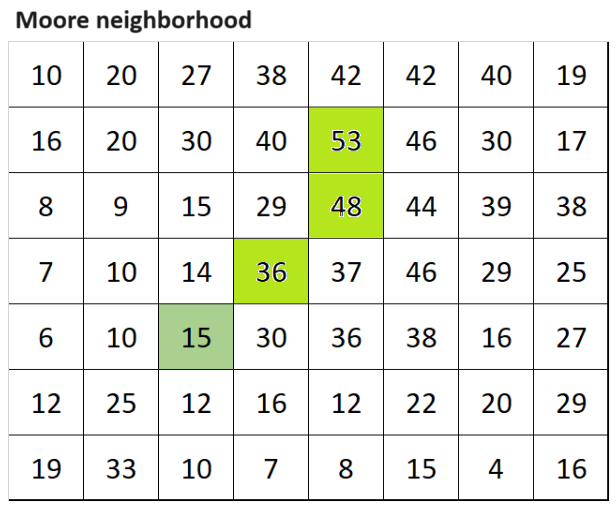
\includegraphics[width=0.6\textwidth]{moore}}

Tento algoritmus sa dostal do políčka s hodnotou 53, ktoré už nemá suseda s väčšou hodnotou. Na to aby sa na dané políčko dostal potreboval 4 iterácie.
\\

Ak spustíme algoritmus využívajúc Von Neumannovu definíciu susedov, tak sa v druhom kroku dostane do situácie keď existujú dvaja maximálny susedia, v závislosti od toho ktorého si algoritmus vyberie záleží výsledná hodnota nájdeného maxima aj počet krokov. 

\centerline{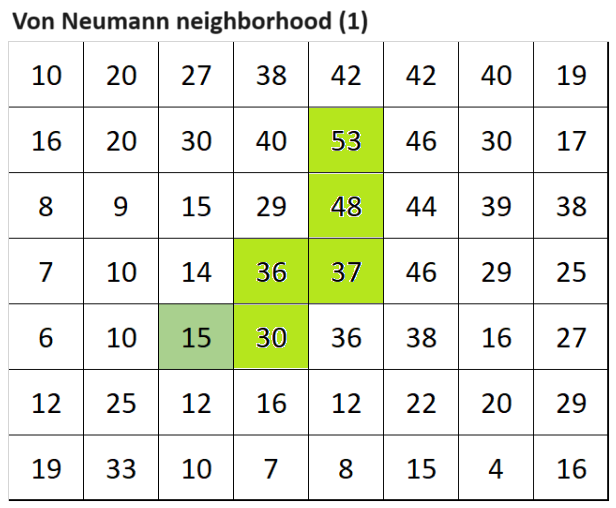
\includegraphics[width=0.6\textwidth]{von_1}}

Vidíme, že pri prvom výbere sa dostane do políčka s hodnotou 53 na 5 krokov.

\centerline{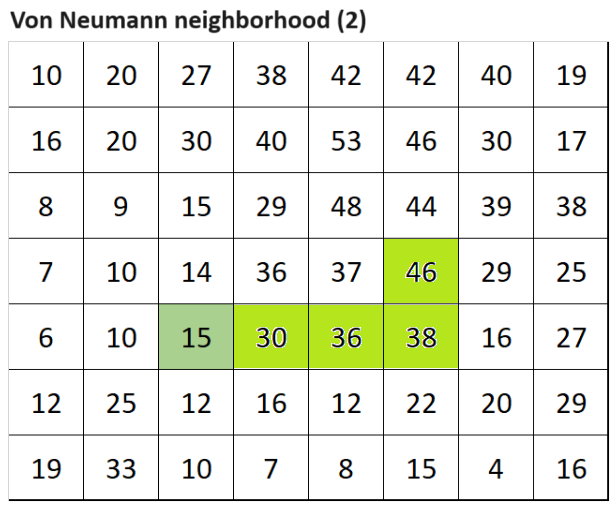
\includegraphics[width=0.6\textwidth]{von_2}} 

Druhý prípad skončí v hodnote 46 po 4 krokoch.
\\

To či tento algoritmus považujeme za deterministický alebo stochastický záleží podľa toho ako sa zachová v situácii keď 2 rôzne kroky vyzerajú lokálne rovnako dobré. Ak si z nich algoritmus vyberá náhodne ide o stochastický algoritmus, ak má povedanú postupnosť v akej má susedov vyberať (napríklad v smere hodinových ručičiek počnúc konkrétnym smerom), ide o deterministický algoritmus. 

\end{document}